\chapter{Desarrollo}

\section{Simule el sistema de control de disparo del SCR mediante un microcontrolador con una entrada de control (potenciómetro o terminal serie), que sea capaz de controlar el	ángulo entre los valores de 50° $\leq$  $\alpha$ $\leq$ 110°}

Para la simulación del esquema trifásico y su control, se hizo uso de la herramienta Proteus en su versión 8.13 en agregado con el añadido de la librería simulino para para poder emular el microcontrolador Arduino, esta representación se muestra en la figura \ref{fig:sim-rec-controlado-trifasico-media-onda} en la cual además se simula un circuito detector de cruce por cero para poder sincronizar los pulsos de activación para los tiristores.

\begin{figure}[h]
	\centering
	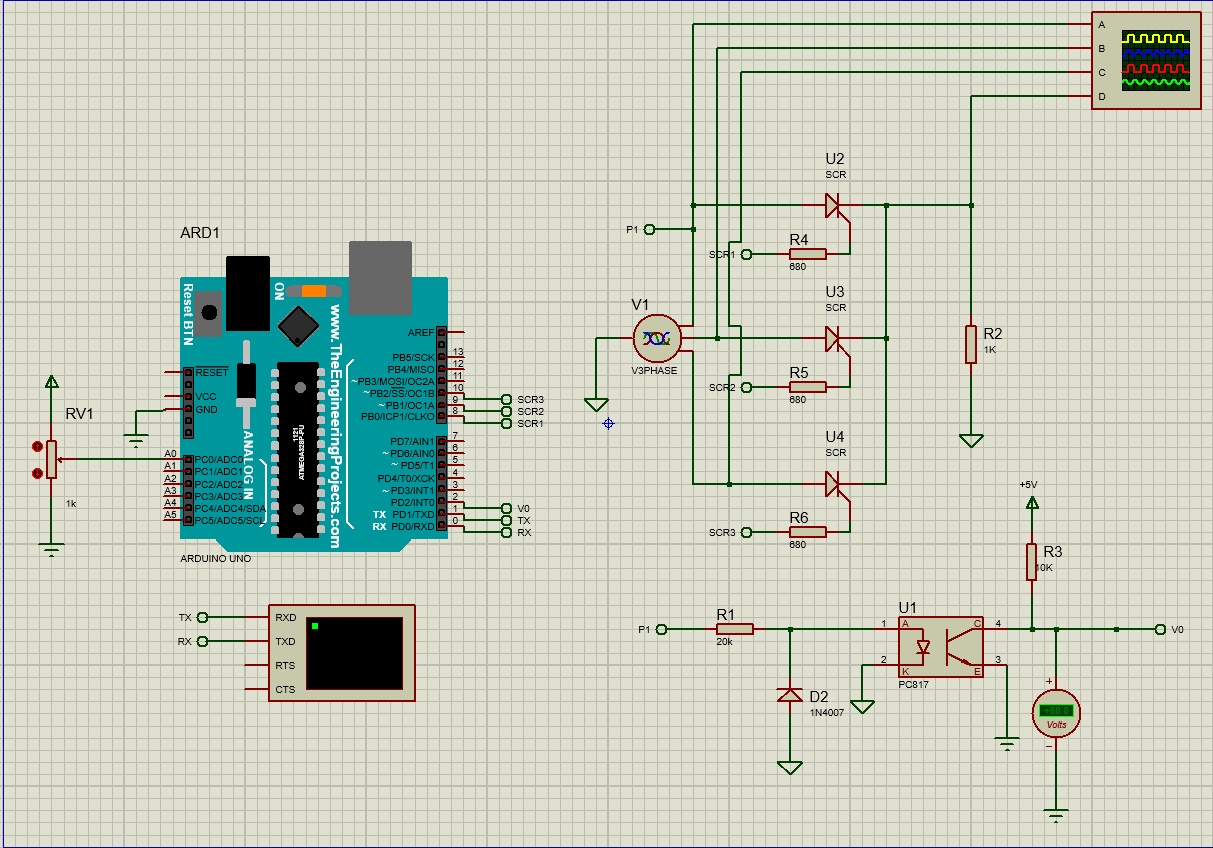
\includegraphics[width=0.7\linewidth]{media/sim-rec-controlado-trifasico-media-onda}
	\caption{Simulación rectificador trifásico media onda}
	\label{fig:sim-rec-controlado-trifasico-media-onda}
\end{figure}

En la parte de control con Arduino se tomo en cuenta el uso de la comunicación serial para definir el angulo de disparo en este caso en su oscilación entre 50 y 110 grados, este método en comparación al uso del potenciometro permite definir con mayor exactitud en ángulo debido a que elimina la incertidumbre en buscar la correcta posición en el giro de la resistencia variable para definir un ángulo de disparo.

\subsection{Parámetros eléctricos de disparo para el tiristor}

En la experiencia 04 se caracterizo el comportamiento del tiristor obteniendo de la misma un voltaje de 0.679V y una corriente de 4.209mA y las cuales se tuvieron en cuenta para el diseño esquemático en la simulación considerando además la salida de voltaje en los pines digitales del microcontrolador a 5V.

\section{Respuesta de la simulación planteada}

\subsection{$\alpha = 50º$}

\begin{figure}[h]
	\centering
	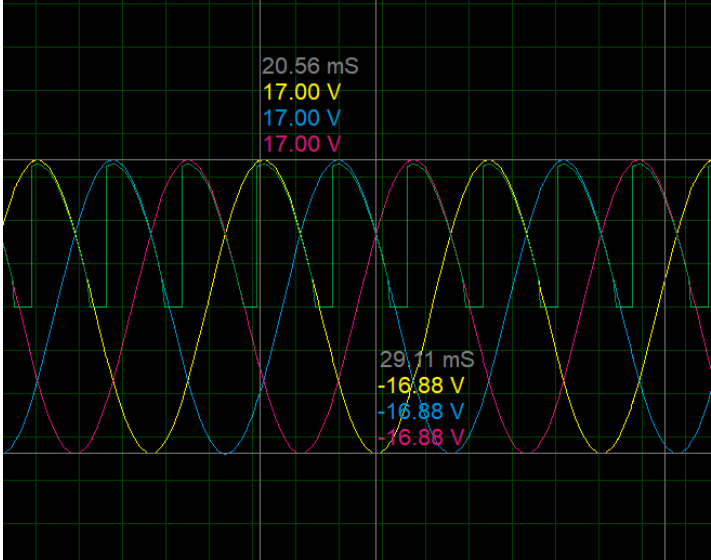
\includegraphics[width=0.7\linewidth]{media/salida-rect-50}
	\caption{Salida rectificada para un angulo de disparo de 50º}
	\label{fig:salida-rect-50}
\end{figure}

\subsection{$\alpha = 110º$}

\begin{figure}
	\centering
	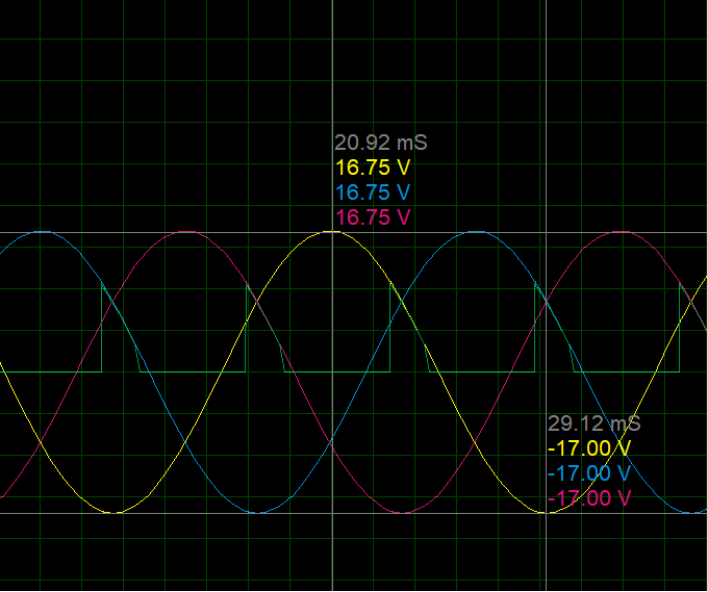
\includegraphics[width=0.7\linewidth]{media/salida-rect-110}
	\caption{Salida rectificada para un angulo de disparo de 110º}
	\label{fig:salida-rect-110}
\end{figure}

